\documentclass[9pt]{beamer}
\usepackage{xeCJK}
\usepackage{ctex}
\usepackage{amsmath}
\usepackage{amssymb}
\usepackage{graphicx}
\usepackage{float}
\usepackage{subfigure}
\setsansfont{Ubuntu Mono}
\setCJKmonofont{AR PL UKai CN}
\usetheme{metropolis}
\title{Solution}
\date{\today}
\author{ljfcnyali \&  CraZYali}
\begin{document}

  \maketitle
  
  \section{easiest}

  \begin{frame}{easiest}
    \onslide<1-> 记$f_i$表示从$i$向右最近的为被删除的元素(初始为$i$)
    
    \onslide<2-> 那么每次操作对存在的元素暴力修改,不存在的用并查集快速跳过即可做到线性
  \end{frame}

  \section{matrix}

  \begin{frame}{matrix}
    \onslide<1-> 类比$\frac{1}{1-x}=\sum_{i}x^i$,将$A$代入该式,发现当且仅当$A^{\infty}$收敛为0时满足该式
    
    \onslide<2-> 由给出的矩阵容易发现,该矩阵一定收敛,所以问题转化为若$A_{i,j}>0$,则连一条$i\rightarrow j$的有向边,求连通的点对数

    \onslide<3-> 这是一个经典问题,可以在$O(\frac{n^3}{\omega})$的时间内解决
  \end{frame}

  \section{hippocentaur}

  \begin{frame}{hippocentaur}
    \onslide<1-> 观察题意,如果手玩一下$n=2$的情况或者观察$n^2$和$4n^2$的关系,可以发现其实一个$2\times 2$的矩形只允许放一个$hippocentaur$

    \onslide<2-> 我们将一个$2\times 2$的矩形称为一个基本单元,而一个$hippocentaur$放置的位置按照从左上角开始顺时针方向称为ABCD

    \onslide<3-> 继续观察,发现横着的两个相邻的格子,如果右边的钦定为A,那么左边的也一定为A,否则会出现两个棋子互相攻击的情况,BCD情况类似
  \end{frame}

  \begin{frame}{hippocentaur}
    \begin{figure}[htbp]
      \centering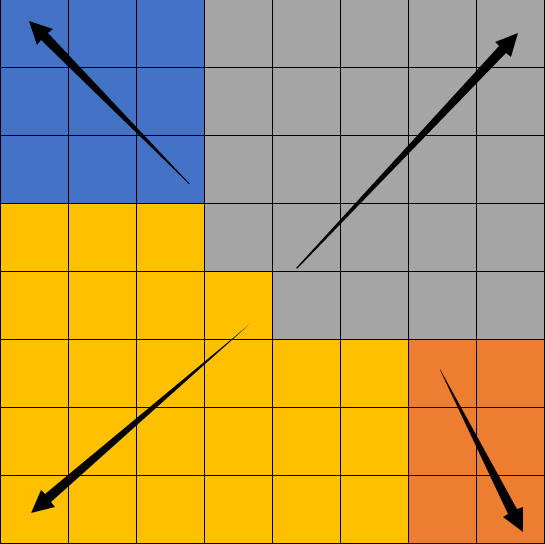
\includegraphics[width=0.8in]{insol.png}
      \end{figure}
    \onslide<1-> 如图所示,那么可以枚举左上角和右下角的两个顶点,得到式子
    \onslide<2->
    \begin{equation}
      \sum_{a=0}^n\sum_{b=0}^n\sum_{c=a}^n\sum_{d=b}^n \binom{c-a+d-b}{c-a}
    \end{equation}
    \onslide<3-> 但是注意到$a=0,b=0$的时候会计算到$a=0,b>0$时的情况,所以需要去重,修改式子后变为
    \onslide<4->
    \begin{equation}
      \sum_{a=1}^{n-1}\sum_{b=1}^{n-1}\sum_{c=a}^{n-1}\sum_{d=b}^{n-1} \binom{c-a+d-b}{c-a}+2\times \sum_{i=0}^{n-1}\sum_{j=0}^{n-1}\binom{i+j}{i}+\binom{n+n}{n}
    \end{equation}
    \onslide<5-> 记(2)式的和为$sum$,再注意到矩形可以旋转90度,而如果两个顶点重合旋转时会算重,所以最后答案为
    \onslide<6->
    \begin{equation}
      ans=2\times sum-(n+1)\times (n+1)
    \end{equation}
  \end{frame}

  \begin{frame}{hippocentaur}
    \onslide<1-> 根据组合恒等式有:
    \onslide<2->
    \begin{equation}
      \sum_{a=0}^{n-1}\sum_{b=0}^{n-1}\binom{a+b}{a}=\binom{n+n}{n}-1
    \end{equation}
    \onslide<3-> 将(2)式的前半部分进行改写
    \onslide<4->
    \begin{equation}
      \begin{aligned}
      &\sum_{a=1}^{n-1}\sum_{b=1}^{n-1}\sum_{c=a}^{n-1}\sum_{d=b}^{n-1}\binom{c-a+d-b}{c-a}\\
      =&\sum_{a=1}^{n-1}\sum_{b=1}^{n-1}\sum_{c=0}^{n-a-1}\sum_{d=0}^{n-b-1}\binom{c+d}{c}\\
      =&\sum_{a=1}^{n-1}\sum_{b=1}^{n-1}\binom{n+a+n-b}{n+a}-1\\
      =&\binom{n+n}{n}-2n-(n-1)^2\\
      =&\binom{n+n}{n}-(n+1)^2
    \end{aligned}
    \end{equation}
  \end{frame}

  \begin{frame}{hippocentaur}
    \onslide<1-> 所以答案可以化简为
    \onslide<2->
    \begin{equation}
      ans=8\binom{n+n}{n}-(3n^2+2n+7)
    \end{equation}
    \onslide<3->求个组合数即可解决全部问题
  \end{frame}
  
  \section{count}

  \begin{frame}{count} 
    \onslide<1-> 定义二元多项式$F(x,y)=\sum_{i=0}^n\sum_{j=0}^m a_{i,j}x^iy^j$
    
    \onslide<2-> 设系数$a_{i,j}$表示一个大小为$i$的连通图,往外连$j$条边的方案数,$a_{i,j}=\frac{g_i}{i!}\binom{i}{j}$,其中$g_i$表示$i$个点的连通图方案数。那么$e^F$的$x^{n-1}y^k$系数就是1号点度数为$k$的方案数,求和即可

    \onslide<3-> 因为二元多项式$exp$并没有作为考点的必要,所以数据范围设为暴力乘的复杂度,为$O(nk^2(log_2k+log_2 n))$
  \end{frame}
  
  \section{Thanks}

\end{document}
